% !TEX root = ../main.tex

\chapter{FlashTOD 检测模型与数据集准备}

\section{金融异常检测任务建模}

金融大规模异常检测任务的本质，是在高维、多源、强时序的交易与行为数据中，快速识别少量偏离正常模式的高风险样本。与一般的二分类任务不同，这类任务不仅受到标签稀缺、样本极度不平衡等问题影响，还直接受制于系统吞吐、响应时延和设备资源约束。从工程实现角度看，任务建模不能只停留在输入标签和输出分数的概念层面，还必须明确原始金融数据如何进入系统、哪些对象进入候选召回、评分阶段对输入提出什么接口要求，以及输出结果如何支持后续排序、复核与追踪。本文在对金融大规模数据异常检测任务进行任务建模时，有以下考虑。

从输入形式上看，本文将待检测对象抽象为一个由样本集合 $X=\{x_1,x_2,\ldots,x_n\}$ 组成的金融行为数据集，其中每个样本 $x_i$ 对应一条交易记录、一个账户时间窗行为摘要或一个节点行为表示。每个样本由连续型数值特征、离散型类别特征和时间上下文特征组成，在预处理阶段被统一映射为固定维度向量表示 $v_i\in\mathbb{R}^d$。对于图结构金融数据，还需将节点特征与边关系经时间窗统计、邻域聚合或嵌入映射后转换为向量化表示，从而与表格型交易数据形成统一输入接口\citep{dgraphfin_paper}。这一抽象为候选召回模块和异常评分模块提供一致的向量接口，使交易级异常、账户级异常与图节点级异常能够进入同一条执行链路。

从系统目标上看，本文的异常检测任务采用``候选召回---异常评分''两阶段处理框架。全量评分在大规模数据条件下会同时放大距离计算、邻域组织和中间结果存储开销，因此先通过候选召回把评分对象压缩到规模可控的局部邻域，再由 PyTOD 异常评分模块完成更细粒度的异常判断。第一阶段利用高吞吐近似最近邻检索在大规模样本中快速找到与查询样本最相关的候选集合 $C_i$；第二阶段利用 PyTOD 在候选集合上执行张量化异常评分，生成异常分数 $s_i$。形式上，可将系统目标写为
\begin{equation}
  C_i = \mathcal{R}(v_i, \mathcal{I}), \qquad s_i = \mathcal{F}(v_i, C_i),
  \label{eq:flash-tod-task-model}
\end{equation}
式~\eqref{eq:flash-tod-task-model} 中，$\mathcal{R}$ 表示候选召回过程，$\mathcal{I}$ 表示候选索引，$\mathcal{F}$ 表示异常评分函数。系统最终性能由候选召回质量、候选规模控制和评分阶段执行效率共同决定。因此，本文将两阶段结构作为系统建模基础\citep{zhao2022tod}。

从输出形式上看，系统可产生三类结果：用于后续阈值判断或人工复核排序的每个样本的异常分数，用于构造重点审查名单的 Top-$k$ 风险样本集合，以及用于系统追踪和后续解释分析的与异常结果相关的候选邻域、关键特征统计及日志信息。在金融风控场景中，这三类结果分别对应在线筛查、风险排序和审计追踪三种实际需求。

图~\ref{fig:fin-ad-model} 对这一统一任务建模过程进行了整体展示。

\begin{figure}[!htbp]
  \centering
  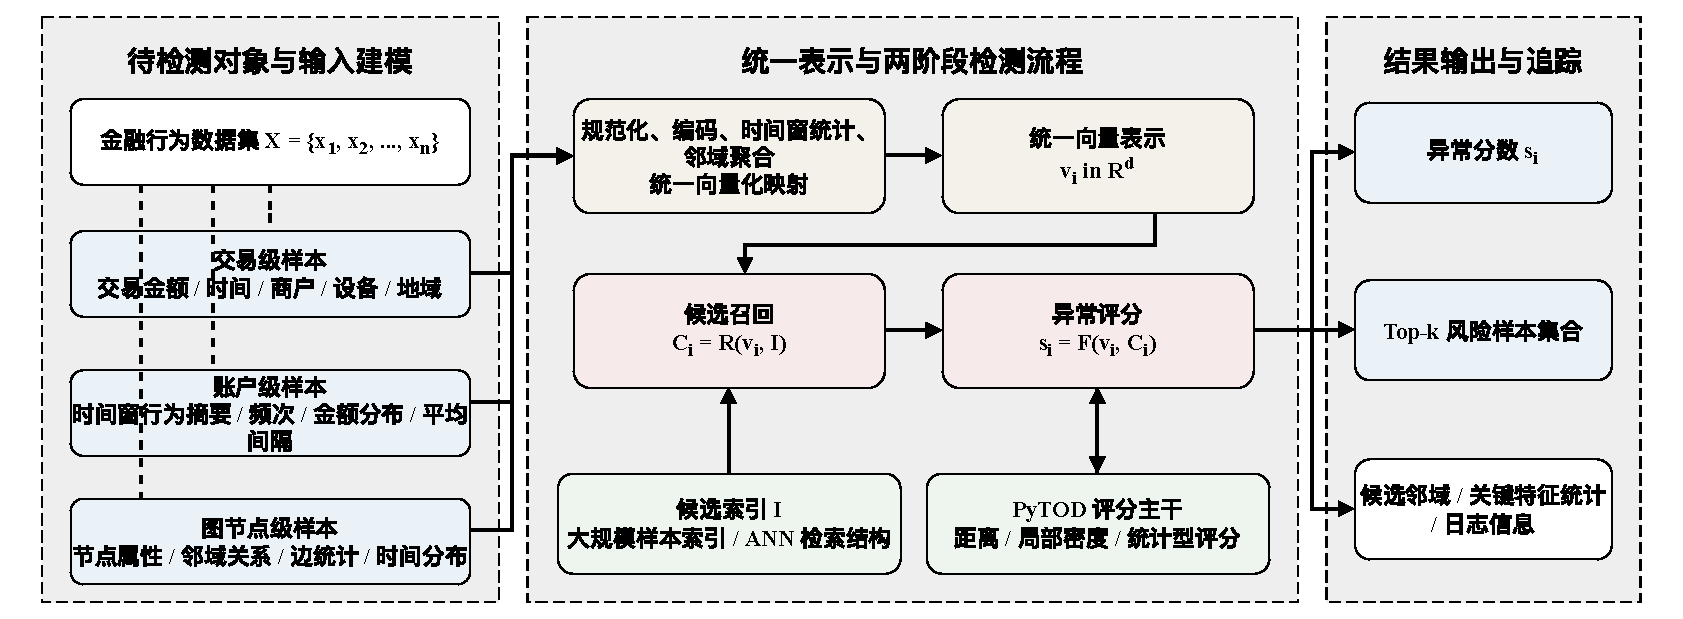
\includegraphics[width=\linewidth]{figures/fig3-1_financial_anomaly_task_model.pdf}
  \caption{金融异常检测任务建模图（本文绘制）}
  \label{fig:fin-ad-model}
\end{figure}

在该统一建模下，单笔交易记录、账户时间窗摘要和图节点邻域信息均映射为固定维度向量 $v_i\in\mathbb{R}^d$，共用一套输入接口。候选召回与 PyTOD 评分据此共享输入，输出也自然收束为异常分数、Top-$k$ 风险对象以及必要的候选邻域和日志信息。

\section{FlashTOD 系统整体架构}

在向量化表示—候选召回—异常评分—结果输出与追踪这一处理链路上，本文选择由 PyTOD 与 FlashANNS 协同构成的异常检测系统作为具体研究对象，并将其命名为 FlashTOD。PyTOD 将异常检测过程抽象为可复用的张量算子，适合作为异常评分模块；FlashANNS 本身是高吞吐 ANNS 系统，在本文中被组织为候选召回前端，如图~\ref{fig:pytod-flashanns-concept} 所示。二者的角色分工相对清晰，但真正落到工程实现时，阶段边界上的开销并不会因为模块职责明确而自动消失。若查询特征先在 CPU 上构造，再传输至 GPU 检索，而候选结果又回到 CPU 重新组织后再送回 GPU 评分，那么瓶颈会很快转移到 CPU$\leftrightarrow$GPU 数据搬运与阶段同步上；进一步地，在多 GPU 场景中，若将多个 GPU 的局部结果重新集中到 CPU 归并，CPU 还可能再次成为系统瓶颈。

FlashTOD 的总体结构可以划分为输入与特征构造、候选召回、异常评分、GPU 执行支撑、多 GPU 扩展和结果输出几个层次。系统重点组织 PyTOD 与 FlashANNS 之间的数据流、候选接口和执行边界，使候选召回与异常评分能够在统一系统链路中协同工作。图~\ref{fig:pytod-flashanns-concept} 中 FAISS-GPU 表示前期 ANN 接口和设备侧检索路径的初步验证组件；完整 FlashTOD 路径中的主要候选召回前端为 FlashANNS。

在输入层，系统接收金融交易记录、账户行为摘要、设备信息以及关系特征等多源数据；在预处理层，这些异构输入经过缺失值处理、类别编码、时间窗统计、图关系聚合和归一化后，被统一映射为固定维度向量表示 $v_i\in\mathbb{R}^{d}$。这一统一向量既是候选召回模块的检索输入，也是后续 PyTOD 评分阶段的基础对象，从而避免为不同数据来源分别维护割裂的执行接口。

在候选召回层，完整 FlashTOD 路径以 FlashANNS 作为主要候选召回前端，面向大规模外存近似最近邻检索提供高吞吐候选生成路径；FAISS-GPU 则主要用于前期验证显存内或局部索引场景下的候选召回接口、设备侧输入输出路径以及候选 ID 与距离返回格式。候选召回层输出候选 ID、局部距离、排序信息以及后续评分所需的数据引用。在异常评分层，PyTOD 接收查询向量与候选集合，在候选范围内完成距离计算、局部密度或统计聚合等张量化异常评分，并生成异常分数。

在数据路径层，FlashTOD 尽量让查询表示、候选缓冲和评分中间张量保持 GPU 常驻，只在原始输入、必要日志和最终结果等边界通过页锁定内存（pinned memory）与主机交互，以压缩 CPU--GPU 数据往返和阶段同步开销。在多 GPU 扩展层，系统优先采用索引复制（replicated）架构，使每张 GPU 独立完成本地候选召回与异常评分闭环；当索引容量或部署条件限制完整复制时，再进入设备侧归并（GPU merge）或主机侧聚合（CPU aggregation）等兜底路径。最终输出层则面向风险排序、异常分数、前 $k$ 个高风险对象（Top-$k$）、日志记录与反馈接口，为后续实验评估和工程监控提供统一结果。

\begin{figure}[!htbp]
  \centering
  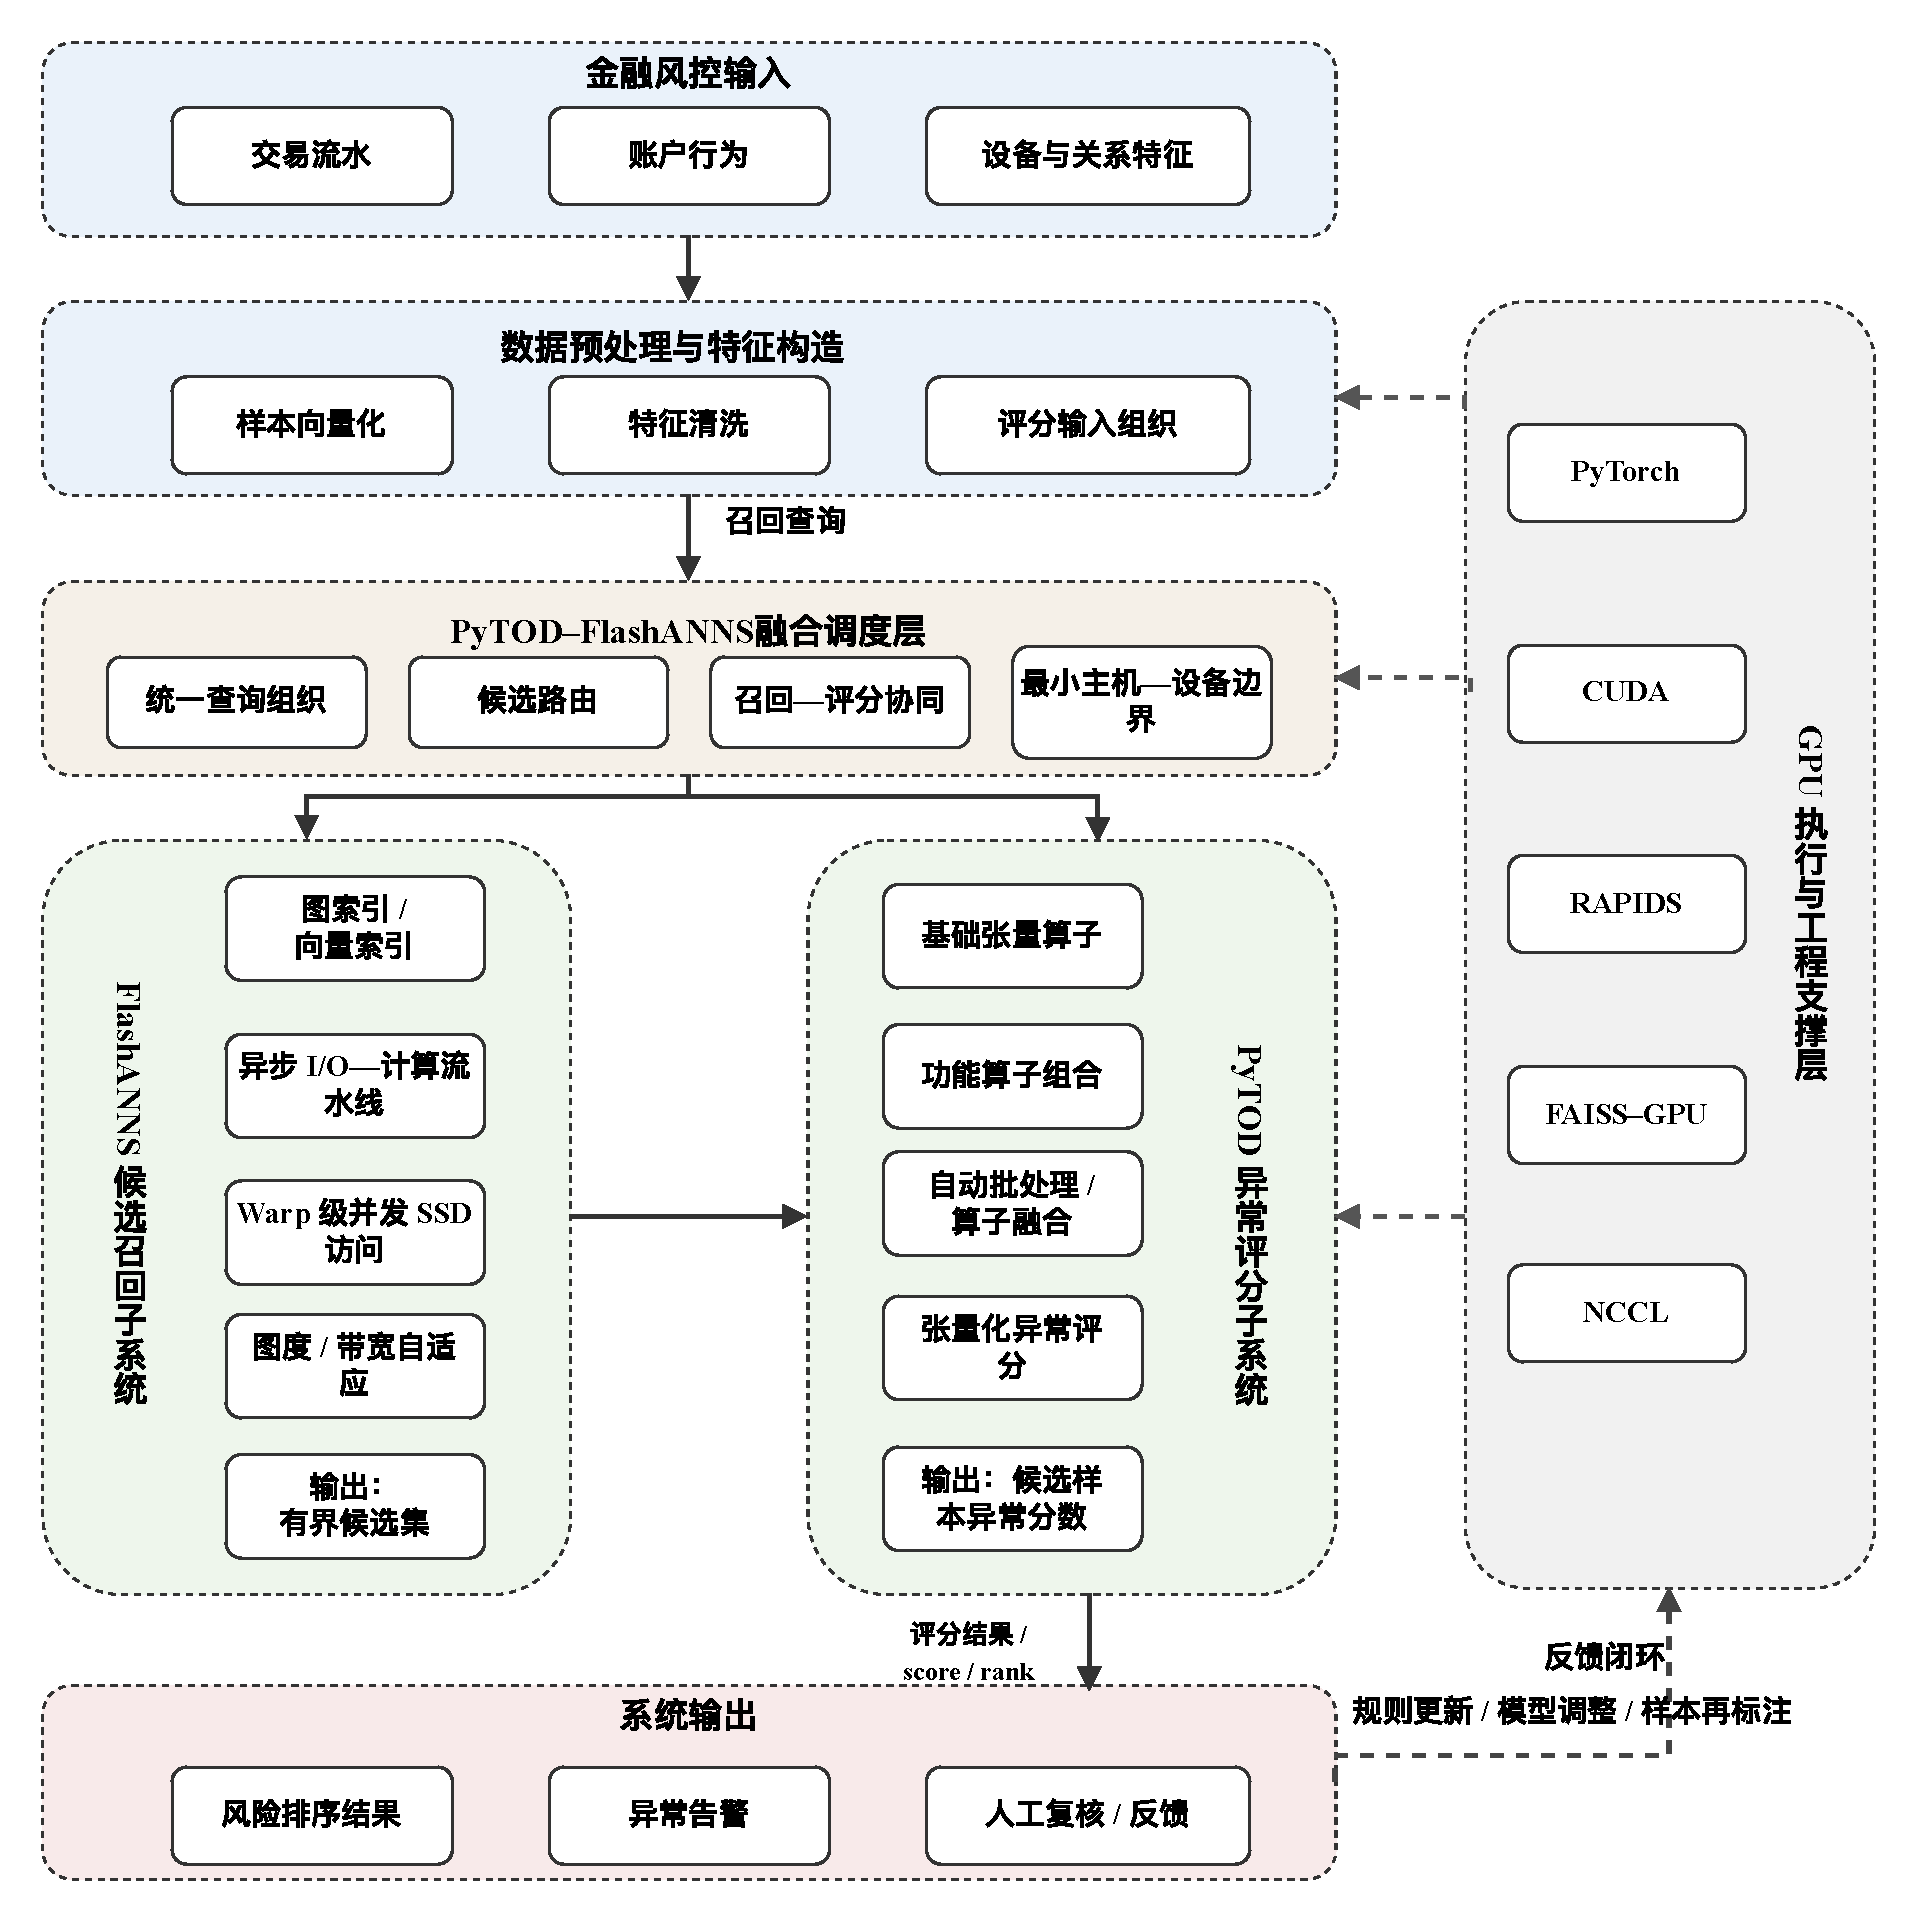
\includegraphics[width=0.95\linewidth]{figures/fig3-2_pytod_flashanns_concept.pdf}
  \caption{FlashTOD 系统概念图（本文绘制）}
  \label{fig:pytod-flashanns-concept}
\end{figure}

\FloatBarrier

\section{实验数据集选取与构建}

本文的数据集安排围绕全文实验口径逐层展开。真实或半真实金融数据承担现实场景下的有效性验证；1M 规模合成数据作为桥接层，用于把真实数据上的方法可用性与后续系统实验接到同一条规模链路上；10M 与 50M 规模合成数据主要对应单卡性能实验；多 GPU 扩展与压力测试则继续延伸到 100M 规模\citep{ibm_aml_data,ibm_amlsim}。下文若无特殊说明，M 均表示样本数量级，1M、10M、50M 和 100M 分别约对应 100 万、1000 万、5000 万和 1 亿条样本。这样安排是为了让真实口径、单卡性能口径和多 GPU 扩展口径之间能够平滑过渡。

本文所称“真实或半真实金融数据”，主要指 IEEE-CIS、Credit Card Fraud Detection、DGraphFin 等公开金融相关数据集。这类数据通常来源于真实业务或真实任务背景，但已经经过脱敏、采样、匿名化、特征变换或竞赛化处理，仍保留金融异常检测中的高维稀疏、类别不平衡、行为偏离和关系结构等典型特征，却不能等同于金融机构生产系统中的在线原始流量。相应地，AMLSim / IBM AML 的 10M、50M、100M 数据主要用于构造可控规模下的压力测试和扩展性验证，适合观察系统吞吐、延迟、I/O 路径和多 GPU 扩展趋势，但不应直接解释为真实生产负载的等比例替代。

在真实口径的有效性验证中，本文主要使用三类公开金融数据。第一类为 IEEE-CIS 欺诈检测数据集（IEEE-CIS Fraud Detection），该数据集包含交易表与身份表两部分，特征维度高、缺失值复杂，较接近现实支付风控场景，适合检验系统在高维结构化金融数据上的向量化表示、候选召回与评分链路是否能够稳定工作\citep{ieee_cis_fraud}。第二类为 Credit Card Fraud Detection 数据集，该数据集虽规模相对较小，但具有经典性和广泛使用基础，适合提供一组较稳定的对照验证口径\citep{dalpozzolo2015creditcard,creditcardfraud_kaggle}。第三类为 DGraphFin 金融图数据集（DGraphFin），其包含大规模节点与边关系以及金融行为特征，主要用于检验图金融数据在经过向量化映射后，能否进入本文统一的候选召回---异常评分链路\citep{dgraphfin_paper,dgraphfin_site,dgraphfin_baseline}。在具体实验组织时，本文将真实数据实验控制在与 1M 合成数据相近的输入量级，以保证有效性验证与后续桥接实验之间的口径连续。

在 1M 规模桥接实验中，本文采用基于 IBM 反洗钱数据与模拟体系（IBM AML / AMLSim）构建的高保真合成金融交易数据。IBM AML-Data 明确以洗钱与异常金融交易为目标，提供带标签的合成金融交易数据集；AMLSim 则能够根据预定义行为规则、账户关系和交易模式生成大规模、可控分布的银行交易数据\citep{ibm_aml_data,ibm_amlsim}。已有研究也使用 AMLSim 构建百万节点量级的反洗钱图，用于分析可扩展图学习路径\citep{weber2018scalableaml}。1M 合成规模用于衔接真实集验证与更大规模系统实验，同时保留金融语境和结构一致性。这类模拟数据便于控制规模和异常模式，但仍不能直接替代真实银行生产流量。

在更大规模的性能与扩展实验中，本文继续沿用 IBM AML / AMLSim 生成的高保真合成数据。10M 与 50M 主要用于单卡性能验证和中大规模趋势观察；多 GPU 路径则在 10M、50M 与 100M 三个层级上继续展开，其中 10M 用于索引复制主方案的起始扩展口径，50M 用于中间规模观察，100M 用于更强的容量与 I/O 压力场景。与简单随机生成数据相比，IBM AML / AMLSim 体系保留了更强的金融语境和结构一致性，因此可作为系统实验的统一规模底座。

不同数据集在全文中的角色由此也更加清晰：IEEE-CIS、Credit Card Fraud Detection 和 DGraphFin 对应真实或半真实数据口径下的有效性验证；1M 合成数据承担真实集与系统实验之间的桥接；10M、50M、100M 合成数据则分别进入单卡性能、多 GPU 扩展和超大规模压力测试。为便于说明不同数据集在全文中的基本属性，表~\ref{tab:datasets-overall} 汇总了数据来源与实验规模口径。

\begin{table}[htbp]
  \caption{实验数据集总体信息}
  \label{tab:datasets-overall}
  \centering
  \small
  \renewcommand{\arraystretch}{1.2}
  \begin{adjustbox}{max width=\linewidth}
  \begin{tabular}{P{2.8cm}P{2.6cm}P{4.0cm}P{2.3cm}P{2.6cm}P{4.1cm}}
    \toprule
    数据集 & 来源类型 & 数据形态 & 实验规模口径 & 标签形式 & 在本文中的用途\\
    \midrule
    IEEE-CIS Fraud Detection & 真实/半真实公开金融数据 & 结构化交易表 + 身份表，高维表格特征、缺失值较复杂 & 约 1M 级输入口径 & 二分类欺诈标签 & 真实场景下的主有效性验证，检验系统在高维金融表格数据上的可用性\\
    Credit Card Fraud Detection & 真实/半真实公开金融数据 & 结构化信用卡交易表格，经典欺诈检测基准 & 按统一实验口径组织到约 1M 级输入 & 二分类欺诈标签 & 作为经典基准数据集，用于对照验证两阶段框架的有效性\\
    DGraphFin & 真实/半真实公开金融图数据 & 图节点、边关系及金融行为特征 & 约 1M 级输入口径 & 节点/行为异常标签 & 验证图金融数据在向量化映射后进入统一候选召回---异常评分链路的可行性\\
    IBM AML / AMLSim（1M） & 高保真合成金融交易数据 & 合成账户---交易网络与表格化交易记录 & 1M & 异常交易/可疑行为标签 & 真实集与系统实验之间的桥接规模，用于统一后续单卡与多 GPU 实验口径\\
    IBM AML / AMLSim（10M） & 高保真合成金融交易数据 & 合成账户---交易网络与表格化交易记录 & 10M & 异常交易/可疑行为标签 & 单卡性能验证主规模，同时作为多 GPU 索引复制扩展起始规模\\
    IBM AML / AMLSim（50M） & 高保真合成金融交易数据 & 合成账户---交易网络与表格化交易记录 & 50M & 异常交易/可疑行为标签 & 单卡中大规模性能验证与多 GPU 中间规模扩展观察\\
    IBM AML / AMLSim（100M） & 高保真合成金融交易数据 & 合成账户---交易网络与表格化交易记录 & 100M & 异常交易/可疑行为标签 & 多 GPU 归并、I/O 路径与超大规模压力测试\\
    \bottomrule
  \end{tabular}
  \end{adjustbox}
\end{table}

\begin{table}[htbp]
  \caption{数据集属性与实验用途说明}
  \label{tab:dataset-stats-usage}
  \centering
  \footnotesize
  \setlength{\tabcolsep}{2.0pt}
  \renewcommand{\arraystretch}{1.18}
  \begin{adjustbox}{max width=\linewidth}
  \begin{tabular}{P{2.45cm}P{3.1cm}P{1.75cm}P{3.3cm}P{3.0cm}P{3.4cm}}
    \toprule
    数据集 & 数据来源与属性 & 规模口径 & 原始特征说明 & 统一表示口径 & 本文用途\\
    \midrule
    IEEE-CIS Fraud Detection & 公开金融欺诈任务数据，经竞赛化与特征脱敏处理 & 约 1M 级输入口径 & 交易表与身份表合并后约 434 列，去除 ID 与标签后的字段数随预处理变化 & 预处理后映射为固定维度向量 $v_i\in\mathbb{R}^{d}$ & 真实或半真实口径下的高维表格有效性验证\\
    Credit Card Fraud Detection & 公开信用卡交易欺诈数据，特征经匿名化变换 & 约 1M 级输入口径 & 30 个输入特征，包括匿名化主成分、交易时间与金额 & 预处理后映射为固定维度向量 $v_i\in\mathbb{R}^{d}$ & 经典金融欺诈基准上的对照验证\\
    DGraphFin & 公开金融图任务数据，包含节点、边关系与行为特征 & 约 1M 级输入口径 & 17 维节点原始属性，并结合边关系与邻域行为统计 & 节点及邻域信息聚合为固定维度向量 $v_i\in\mathbb{R}^{d}$ & 图金融数据向量化后进入统一链路的有效性验证\\
    IBM AML / AMLSim（1M） & 高保真合成金融交易数据，标签与异常比例随生成配置确定 & 1M & 合成账户、交易网络与表格化交易记录 & 预处理后映射为固定维度向量 $v_i\in\mathbb{R}^{d}$ & 真实口径与系统性能实验之间的桥接规模\\
    IBM AML / AMLSim（10M） & 高保真合成金融交易数据，主要放大样本规模 & 10M & 合成账户、交易网络与表格化交易记录 & 预处理后映射为固定维度向量 $v_i\in\mathbb{R}^{d}$ & 单卡性能验证与多 GPU 索引复制起始规模\\
    IBM AML / AMLSim（50M） & 高保真合成金融交易数据，强化中大规模路径压力 & 50M & 合成账户、交易网络与表格化交易记录 & 预处理后映射为固定维度向量 $v_i\in\mathbb{R}^{d}$ & 单卡中大规模趋势与多 GPU 中间规模观察\\
    IBM AML / AMLSim（100M） & 高保真合成金融交易数据，用于更强容量与 I/O 压力 & 100M & 合成账户、交易网络与表格化交易记录 & 预处理后映射为固定维度向量 $v_i\in\mathbb{R}^{d}$ & 多 GPU 归并、共享路径冲突与压力测试\\
    \bottomrule
  \end{tabular}
  \end{adjustbox}
\end{table}

\textit{数据集名称口径说明：}需要说明的是，表中公开数据集名称、实验导出文件名和预处理后向量维度并不完全等同。部分实验文件来自公开数据集的预处理导出结果，部分文件来自 AMLSim 或金融合成数据生成流程。为避免将原始字段维度与预处理后向量维度混淆，本文在表中分别列出原始数据来源、实验文件名、统一向量维度和实验用途。其中，fraud / ADBench 13\_fraud 对应 ADBench 中的 fraud 导出文件，作为公开金融欺诈数据的预处理实验口径；campaign / ADBench 5\_campaign 为 ADBench 公开异常检测数据；fraud\_handbook 来源于金融欺诈样例与合成链路；amlsim 对应 IBM AML / AMLSim 生成配置；finance\_seed\_200k 为合成种子或中间调试数据，不作为最终主实验规模。IEEE-CIS 与 DGraphFin 在正文中用于说明真实或半真实金融数据来源和图金融口径，但当前显存估算表只覆盖已经导出的向量文件，因此未单独列入。

\begin{table}[htbp]
  \caption*{表~\ref{tab:dataset-stats-usage} 补充：当前已导出实验文件的向量维度与全量距离计算显存估算}
  \centering
  \footnotesize
  \setlength{\tabcolsep}{2.2pt}
  \renewcommand{\arraystretch}{1.12}
  \begin{adjustbox}{max width=\linewidth}
  \begin{tabular}{P{3.4cm}P{1.6cm}P{1.0cm}P{1.7cm}P{2.1cm}P{2.3cm}P{3.0cm}}
    \toprule
    数据集或规模 & 样本数 $n$ & 维度 $d$ & 输入矩阵 & 距离矩阵 $n^2$ & 显式差分 $n^2d$ & 说明\\
    \midrule
    fraud / ADBench 13\_fraud & 284807 & 29 & 31.5\,MiB & 302\,GiB & 8.56\,TiB & 真实集，全量距离矩阵已超单卡显存\\
    campaign / ADBench 5\_campaign & 41188 & 62 & 9.74\,MiB & 6.32\,GiB & 392\,GiB & 输入很小，但显式成对差分仍不可取\\
    fraud\_handbook（1M） & 1M & 20 & 76.3\,MiB & 3.64\,TiB & 72.8\,TiB & 合成桥接规模\\
    fraud\_handbook（10M） & 10M & 20 & 763\,MiB & 364\,TiB & 7.11\,PiB & 单卡与多 GPU 起始性能规模\\
    fraud\_handbook（50M） & 50M & 20 & 3.73\,GiB & 8.88\,PiB & 178\,PiB & 中大规模压力场景\\
    fraud\_handbook（100M） & 100M & 20 & 7.45\,GiB & 35.5\,PiB & 711\,PiB & 超大规模压力场景\\
    amlsim（1M） & 1M & 9 & 34.3\,MiB & 3.64\,TiB & 32.7\,TiB & 合成桥接规模\\
    amlsim（10M） & 10M & 9 & 343\,MiB & 364\,TiB & 3.20\,PiB & 中大规模性能场景\\
    amlsim（100M） & 100M & 9 & 3.35\,GiB & 35.5\,PiB & 320\,PiB & 超大规模压力场景\\
    finance\_seed\_200k & 200k & 20 & 15.3\,MiB & 149\,GiB & 2.91\,TiB & 合成种子或中间数据\\
    \midrule
    \multicolumn{7}{P{15.1cm}}{\footnotesize 注：估算均按 \texttt{float32} 计算。输入矩阵按 $4nd$ 字节估算；距离矩阵按 $4n^2$ 字节估算，可视为直接保留全量样本两两距离的最低存储量级；显式差分按 $4n^2d$ 字节估算，用于说明朴素成对差分中间张量的显存风险。实际 PyTOD/TOD 实现会通过批处理、算子组织或候选召回缩小计算范围，本文不将该估算解释为实际运行时固定占用。}\\
    \bottomrule
  \end{tabular}
  \end{adjustbox}
\end{table}

\textit{说明：}公开金融数据集的原始字段维度与进入 FlashTOD 后的统一向量维度并不等同。不同数据集在缺失值、类别编码、数值归一化和图关系聚合方式上存在差异，本文实验在预处理后将其统一映射为固定维度向量 $v_i\in\mathbb{R}^{d}$，作为候选召回和异常评分的共同输入；当前实现中各实验数据的向量维度及全量距离计算显存风险见表~\ref{tab:dataset-stats-usage} 的补充说明。IBM AML / AMLSim 高保真合成数据主要用于吞吐、延迟和扩展性压力测试，不等同于真实金融机构生产流量。

这种安排将真实有效性验证与系统压力实验分开：IEEE-CIS、Credit Card Fraud Detection 和 DGraphFin 检验两阶段框架在真实或半真实金融数据上的可用性，1M IBM AML / AMLSim 衔接真实口径和合成规模，后续更大样本层级则逐步进入单卡性能、多 GPU 扩展和压力测试。

\FloatBarrier

\section{数据预处理与特征构造}

由于不同数据集在字段命名、数据类型、缺失值比例、标签分布以及时间粒度上存在较大差异，原始金融数据无法直接输入候选召回和异常评分模块。FlashTOD 通过统一向量接口组织数据预处理与特征构造，使处理结果能够同时服务于候选召回和异常评分。本节将进一步讨论，如何在尽量保留业务语义的前提下，将表格型金融数据和图结构金融数据整理为可检索、可评分、可批处理的向量表示 $v_i\in\mathbb{R}^d$。其中，$d$ 由最终预处理脚本确定，并在候选召回与异常评分实验中保持一致。
% TODO(author): 运行最终预处理脚本输出具体 d，并同步回填表 3-2 与附录B。

对于表格型金融数据，预处理过程主要包括缺失值处理、异常字段清洗、数值归一化、类别编码以及时间字段规范化。缺失值处理方面，针对数值型字段采用均值、中位数或业务合理缺省值进行填补，针对类别型字段则引入专门的缺失标识，以避免无效缺失模式被误当作正常类别。异常字段清洗包括删除重复样本、去除明显无意义标识列、统一金额和时间单位等。对于数值型特征，本文采用标准化或归一化处理，降低金额、频率、时差等不同尺度特征之间的量纲影响；对于类别型字段，则采用 one-hot、频次编码或目标统计前的安全编码方式，以便后续统一映射至数值空间\citep{ieee_cis_fraud,dalpozzolo2015creditcard}。经过这一轮处理后，表格型交易记录将进入统一向量接口，直接服务于候选召回与评分阶段。

对于时间信息，本文采用滑动时间窗和行为统计相结合的方式构造增强特征。以单个账户、设备或商户为中心，在固定时间窗口内统计交易频次、交易金额分布、平均时间间隔、夜间交易比例、跨地域交易切换次数等行为特征，并将其与原始交易字段拼接形成更完整的查询表示。金融异常通常体现为当前行为与历史模式之间的偏离。通过时间窗统计，系统可以在不引入复杂序列模型的前提下，把一部分时序上下文编码到统一向量中，使候选召回与异常评分共享同一组行为特征基础。

对于图金融数据，本文先将图节点与边关系转换为节点级向量表示。具体做法包括：对节点原始属性进行规范化与编码；对邻域中边的数量、方向、金额统计和时间分布等进行聚合；将节点本身属性与邻域统计特征拼接形成统一向量。DGraphFin 等图金融数据经过映射后，可以与表格型交易数据一起进入同一条候选召回---异常评分链路，共用系统主流程的执行接口\citep{dgraphfin_paper}。

本文将数值、时间、类别和图关系特征统一收束为固定维度向量，使不同来源金融数据能够进入同一候选召回与评分接口；字段到派生特征的具体组织见附录B补充表~\ref{tab:feature-engineering}。

\FloatBarrier

\section{PyTOD 异常评分模块设计}

在本文的两阶段异常检测框架中，PyTOD 承担的是候选集合上的异常评分模块角色。它接收的是由候选召回阶段输出的查询向量、候选张量及其索引映射信息，并在这一局部邻域内完成距离计算、近邻排序和异常性聚合，从而生成最终异常分数\citep{zhao2022tod}。这一用法将 PyTOD 放在系统的精细评分位置，从而把评分阶段的计算边界控制在候选预算范围内。

从执行接口上看，候选集合 $C_i$ 一旦产生，查询样本 $v_i$ 与候选集合中的向量就可以直接进入 PyTOD 的计算链路，被组织为批量距离矩阵、局部近邻排序结果与聚合统计结果。PyTOD 评分阶段主要完成四类操作：计算查询样本与候选集合之间的距离；对候选集合按距离进行排序或筛选；对局部距离分布、密度差异或邻域结构执行聚合；根据预定义评分函数输出异常分数。这样组织后，PyTOD 能够成为一个围绕候选集工作的 GPU 评分内核。

在评分指标选择上，为了保证同一套执行路径能够适配不同数据集和业务场景下的异常性定义，本文保留基于距离、局部密度和邻域统计的通用评分接口。本文使用 PyTOD 作为统一评分骨架 ，同时保留可切换评分函数的能力，避免把固定评分公式直接写死在系统中。

本文把 PyTOD 放在候选召回之后，专门负责较小候选集合上的精细评分。TOD/PyTOD 原有的自动批处理和多 GPU 支持继续用于缓解评分复杂度，评分能力本身保持不变。经过这一职责划分，系统优化可以集中考察候选召回与数据路径问题。

图~\ref{fig:pytod-backbone} 给出了 PyTOD 异常评分模块的执行流程，表~\ref{tab:score-ops-map} 对常用评分方式与张量算子映射进行了归纳。

\begin{figure}[!htbp]
  \centering
  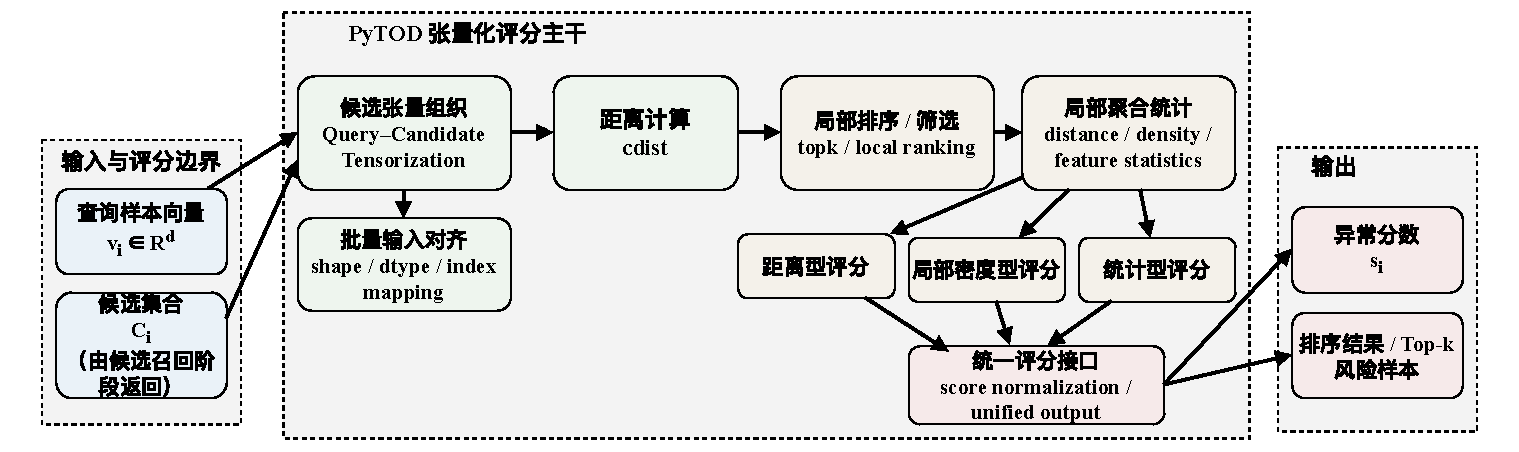
\includegraphics[width=\linewidth]{figures/fig3-3_PyTOD_scoring_backbone.pdf}
  \caption{PyTOD 异常评分模块流程图（本文绘制）}
  \label{fig:pytod-backbone}
\end{figure}

\begin{table}[htbp]
  \caption{异常评分指标与算子映射}
  \label{tab:score-ops-map}
  \centering
  \small
  \renewcommand{\arraystretch}{1.2}
  \begin{adjustbox}{max width=\linewidth}
  \begin{tabular}{P{2.1cm} P{4.0cm} P{3.5cm} P{3.2cm} P{3.7cm}}
    \toprule
    评分类型 & 代表性评分思路 & 候选集上的计算对象 & 简化算子链 & 在本文中的定位\\
    \midrule
    距离型评分 & 依据查询样本与候选邻域的距离分布刻画异常程度 & 查询向量与候选集合的局部距离关系 & \texttt{cdist $\rightarrow$ topk $\rightarrow$ 聚合} & 主评分方式，直观反映样本偏离程度\\
    局部密度型评分 & 比较查询样本与邻域样本的局部密度差异 & 查询样本及其候选邻域的局部密度结构 & \texttt{cdist $\rightarrow$ topk $\rightarrow$ 密度比值} & 补充识别相对异常样本\\
    统计型评分 & 基于候选邻域内特征分布、分位点或边缘偏离程度评分 & 查询样本在候选邻域中的特征偏离情况 & \texttt{统计/直方图 $\rightarrow$ 聚合} & 轻量级辅助评分或对照评分方式\\
    融合评分接口 & 对不同评分结果进行统一输出，形成最终风险排序 & 距离、密度、统计等候选集评分结果 & \texttt{归一化 $\rightarrow$ 加权输出} & 体现统一评分模块的可扩展性\\
    \bottomrule
  \end{tabular}
  \end{adjustbox}
\end{table}

\FloatBarrier

\section{FlashANNS 候选召回前端设计}

在 FlashTOD 中，FlashANNS 负责从大规模样本中快速生成与查询样本最相关的候选集合，为后续精细评分阶段提供规模可控且质量可接受的候选近邻集合\citep{xiao2025flashanns}。这意味着，候选召回模块是评分阶段的前端输入组织模块：它决定了后续 PyTOD 看到什么样的局部邻域、在多大预算下完成评分，以及评分阶段需要承担多大计算负担。

在实现演进上，本文前期利用 FAISS-GPU 较完善的 ANN API 对候选召回接口进行初步验证，主要用于确认查询向量输入、候选 ID 与距离返回、候选集合传递和 PyTOD 候选评分之间的接口关系。随着系统目标转向大规模外存驻留或超显存索引场景，完整 FlashTOD 路径进一步以 FlashANNS 作为主要候选召回前端，以利用其异步 I/O---计算流水线提升大规模候选生成吞吐。

在索引构建阶段，本文以向量化后的样本表示 $v_i$ 为输入，构建面向 ANN 检索的候选索引。对于规模较小且全部可驻留在显存内的实验场景，可直接使用 GPU 端索引完成近似搜索；对于规模更大或需要考虑外存路径的场景，则采用 FlashANNS 异步 I/O---计算流水线所支持的高吞吐检索路径。索引结构和检索路径需要稳定服务于后续评分阶段：既要让查询以较低延迟定位到局部候选邻域，又要保留参数调节空间，使召回质量与系统吞吐之间能够按实验目标进行权衡。

在查询执行阶段，FlashANNS 对输入查询向量 $v_i$ 快速检索并返回一个候选集合 $C_i$。候选集合包含候选 ID、必要的距离值、局部排序信息以及支持后续评分的数据引用。如果这些字段还需要在 CPU 侧进行大规模整理、重排和格式转换，召回阶段获得的吞吐收益就会在模块边界被快速抵消。因此，候选召回模块保持输出格式与评分模块输入接口一致，使候选结果能够直接进入 GPU 评分链路。

在参数组织方面，本文将候选集合规模、召回近邻数量和索引搜索参数统一视为系统预算约束。候选集合过小，可能导致真实异常邻域缺失，从而影响评分质量；候选集合过大，则会使后续 PyTOD 评分重新承受高复杂度负担。类似地，搜索深度过低会使召回不足，过高则会直接侵蚀系统吞吐。因此，参数控制以满足后续异常评分所需的候选质量为目标，使候选召回服务于系统总体约束。

图~\ref{fig:flashanns-workflow} 展示了候选召回模块的基本执行过程，表~\ref{tab:recall-module-params} 总结了关键控制参数。

\begin{figure}[!htbp]
  \centering
  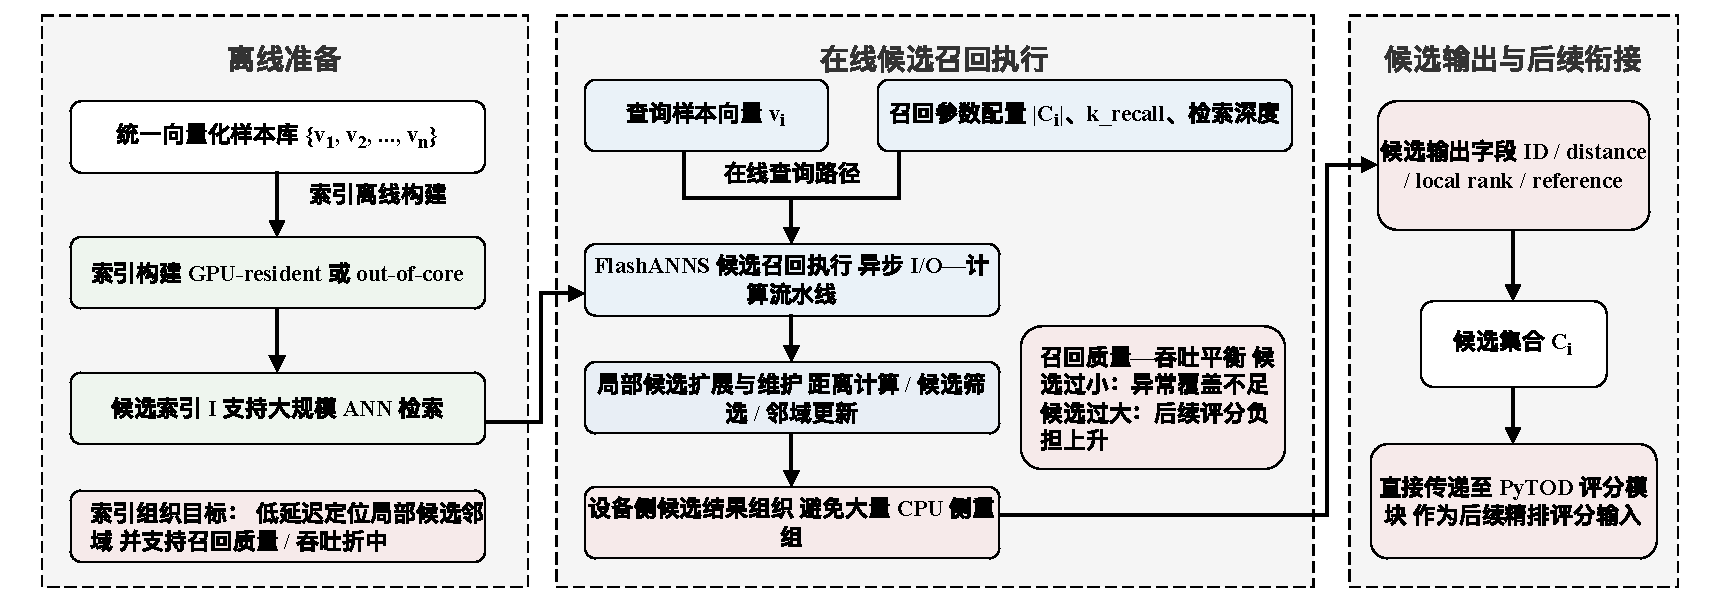
\includegraphics[width=\linewidth]{figures/fig3-4_FlashANNS_candidate_recall_flow.pdf}
  \caption{FlashANNS 候选召回执行流程图（本文绘制）}
  \label{fig:flashanns-workflow}
\end{figure}

\begin{table}[htbp]
  \caption{候选召回模块主要参数}
  \label{tab:recall-module-params}
  \centering
  \small
  \renewcommand{\arraystretch}{1.2}
  \begin{adjustbox}{max width=\linewidth}
  \begin{tabular}{P{2.6cm}P{2.7cm}P{3.2cm}P{4.2cm}P{4.2cm}}
    \toprule
    参数名称 & 符号/表示 & 含义 & 对系统的影响 & 设置原则\\
    \midrule
    候选集合规模 & $|C_i|$ & 每个查询样本返回的候选样本数 & 过小会降低异常覆盖率，过大会增加后续评分负担 & 在召回质量与评分复杂度之间折中设置\\
    近邻返回数量 & $k_{\mathrm{recall}}$ & 候选召回阶段实际返回的近邻数量 & 决定局部邻域完整性与后续评分的输入范围 & 与评分阶段使用的局部邻域规模保持协调\\
    检索深度/访问强度参数 & \texttt{nprobe}、\texttt{efSearch} 等 & 控制 ANN 检索阶段访问的索引范围或搜索强度 & 参数越高通常召回质量更好，但吞吐下降 & 以满足评分需求为目标，而非追求极限检索精度\\
    索引驻留方式 & GPU 常驻（GPU-resident） / 外存驻留（out-of-core） & 候选索引驻留在显存内或通过外存路径访问 & 影响检索延迟、I/O 压力与系统扩展能力 & 小规模优先显存驻留，大规模场景采用外存驻留路径\\
    候选输出字段 & ID、distance、rank、reference & 候选模块返回给评分模块的主要内容 & 决定后续 PyTOD 评分接口是否需要额外重组 & 尽量采用可直接进入 GPU 评分链路的输出格式\\
    查询批大小 & \texttt{batch\_size} & 单次提交到候选召回模块的查询数量 & 影响设备利用率、时延与流水线连续性 & 与 GPU 资源、显存容量和时延约束共同确定\\
    精排预算 & \texttt{rerank\_budget} & 进入高精度评分阶段的候选上限 & 控制精排复杂度与最终检测效果之间的平衡 & 与候选集合规模联动设置，避免全量重评分\\
    \bottomrule
  \end{tabular}
  \end{adjustbox}
\end{table}

\FloatBarrier

\section{FlashTOD 执行流程}

在完成数据预处理、向量化表示、候选召回模块和异常评分模块设计后，本文进一步将二者整合为统一的执行流程。该流程覆盖从查询输入到异常结果输出的完整链路，其目标是在保持模块职责清晰的同时，把各阶段的输入输出接口明确下来，并尽量减少中间结果的重复复制和格式转换。本文将 FlashTOD 的基础执行流程概括为输入向量化、候选召回、候选张量组织、PyTOD 评分和风险输出五个环节。

具体而言，系统接收原始交易记录、账户行为摘要或图节点样本，经由数据预处理与特征构造转换为统一向量表示。随后，向量表示作为查询输入送入候选召回模块：在前期初步验证阶段，该步骤可由 FAISS-GPU 的成熟 ANN API 完成，以验证候选召回与 PyTOD 评分之间的接口；在完整 FlashTOD 路径中，该步骤由 FlashANNS 候选召回前端完成，以支持大规模外存驻留或超显存索引条件下的候选生成。候选集合在 GPU 侧完成必要的组织与重排，形成 PyTOD 可以直接接收的候选张量、距离张量及索引映射结构；PyTOD 在候选集合上执行张量化异常评分，输出异常分数及对应排序结果；最终，系统根据异常分数形成风险样本、日志记录和必要解释信息，并进入后续实验采样或部署监控链路。其中，统一向量接口负责连接异构金融特征与候选召回模块，候选张量组织则负责将候选 ID、距离和排序信息整理为 PyTOD 可直接使用的评分输入。

至此，第三章完成了功能级衔接：系统明确了输入来源、候选生成、评分执行和结果输出方式。当前结果只确认功能可行，数据路径成本仍需进一步压缩。若候选召回结果频繁回传 CPU 再被整理成评分输入，系统链路会重新引入高昂的 CPU$\leftrightarrow$GPU 往返与阶段同步成本；中间结果以 GPU 常驻张量或低开销设备对象表达时，整个候选召回---异常评分过程才更接近统一 GPU 执行链路。因此，第四章继续讨论这条流程在单卡上的数据路径成本。

图~\ref{fig:intermediate-dataflow} 进一步展示查询向量、候选结果与评分中间张量在模块间的传递方式。

\begin{figure}[!htbp]
  \centering
  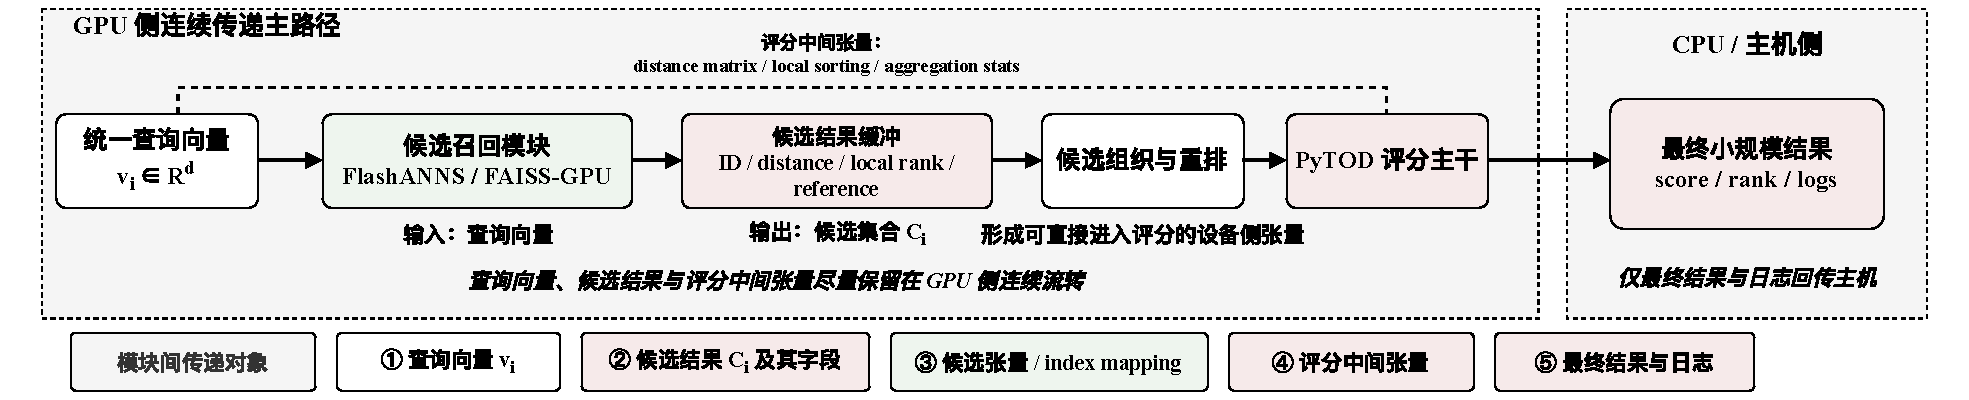
\includegraphics[width=\linewidth]{figures/fig3-5_intermediate_results_transfer.pdf}
  \caption{模块间中间结果传递示意图（本文绘制）}
  \label{fig:intermediate-dataflow}
\end{figure}

图中 FAISS-GPU 表示前期 ANN API 初步验证路径；完整 FlashTOD 路径以 FlashANNS 作为主要候选召回前端。

\FloatBarrier

\section{基础实验与初步验证}

在进入系统级优化和多 GPU 扩展之前，有必要首先验证 FlashTOD 在功能上的正确性，并把真实口径实验与后续 1M 合成桥接实验接到同一条规模链路上。因此，本节的基础实验围绕三个更具体的问题展开：候选召回与异常评分链路是否能够正确联通；在候选集合上执行 PyTOD 评分是否会带来不可接受的检测效果损失；当前初始实现是否已经具备继续进入系统优化阶段的前提。

在功能正确性验证中，实验主要关注查询输入、候选集合生成、候选组织与异常评分输出之间是否存在接口不一致、结果异常或批处理错误。实验安排先以真实或半真实金融数据完成基础联调，再在 1M 合成规模下重复相同口径的检查，以确认候选召回与异常评分接口在跨数据来源条件下仍保持一致。随后，将候选集评分结果与小规模全量评分结果进行比较，以观察候选召回对异常评分口径的影响。实验重点考察精确率—召回率曲线下面积（Precision-Recall Area Under Curve，PR-AUC）、Top-$k$ 召回率（Recall@$k$）和 Top-$k$ 重合度（Top-$k$ overlap）等指标在候选预算受限后的变化，以判断主要排序结果、Top-$k$ 风险样本与整体检测效果是否仍保持在可接受范围内。如果候选集合过小导致异常模式无法被覆盖，则说明候选召回参数仍需调整；如果候选评分与全量评分在主要排序结果上保持较高一致性，则说明两阶段框架具备继续开展系统优化的基础。

基础实验还将初步观察不同数据集下候选召回与异常评分之间的关系。结构化交易数据中的候选召回结果往往对金额、时间和设备行为更敏感，而图金融数据中的候选召回结果则更容易受到邻域统计特征影响。做这一层观察是为了在进入第四章和第五章之前，先确认统一接口和两阶段流程在不同金融数据形态下都能够稳定工作。图~\ref{fig:prelim-effectiveness} 展示了不同数据集上的候选召回---候选评分初步有效性结果。

本节实验以真实或半真实数据和 1M 合成桥接规模为入口，统一采用固定维度向量表示，并以候选集评分对照小规模全量评分。关注重点是候选预算变化对排序一致性、Top-$k$ 风险样本重合度以及 PR-AUC、Recall@$k$ 的影响，从而判断两阶段流程是否足以支撑后续系统优化。

\begin{figure}[!htbp]
  \centering
  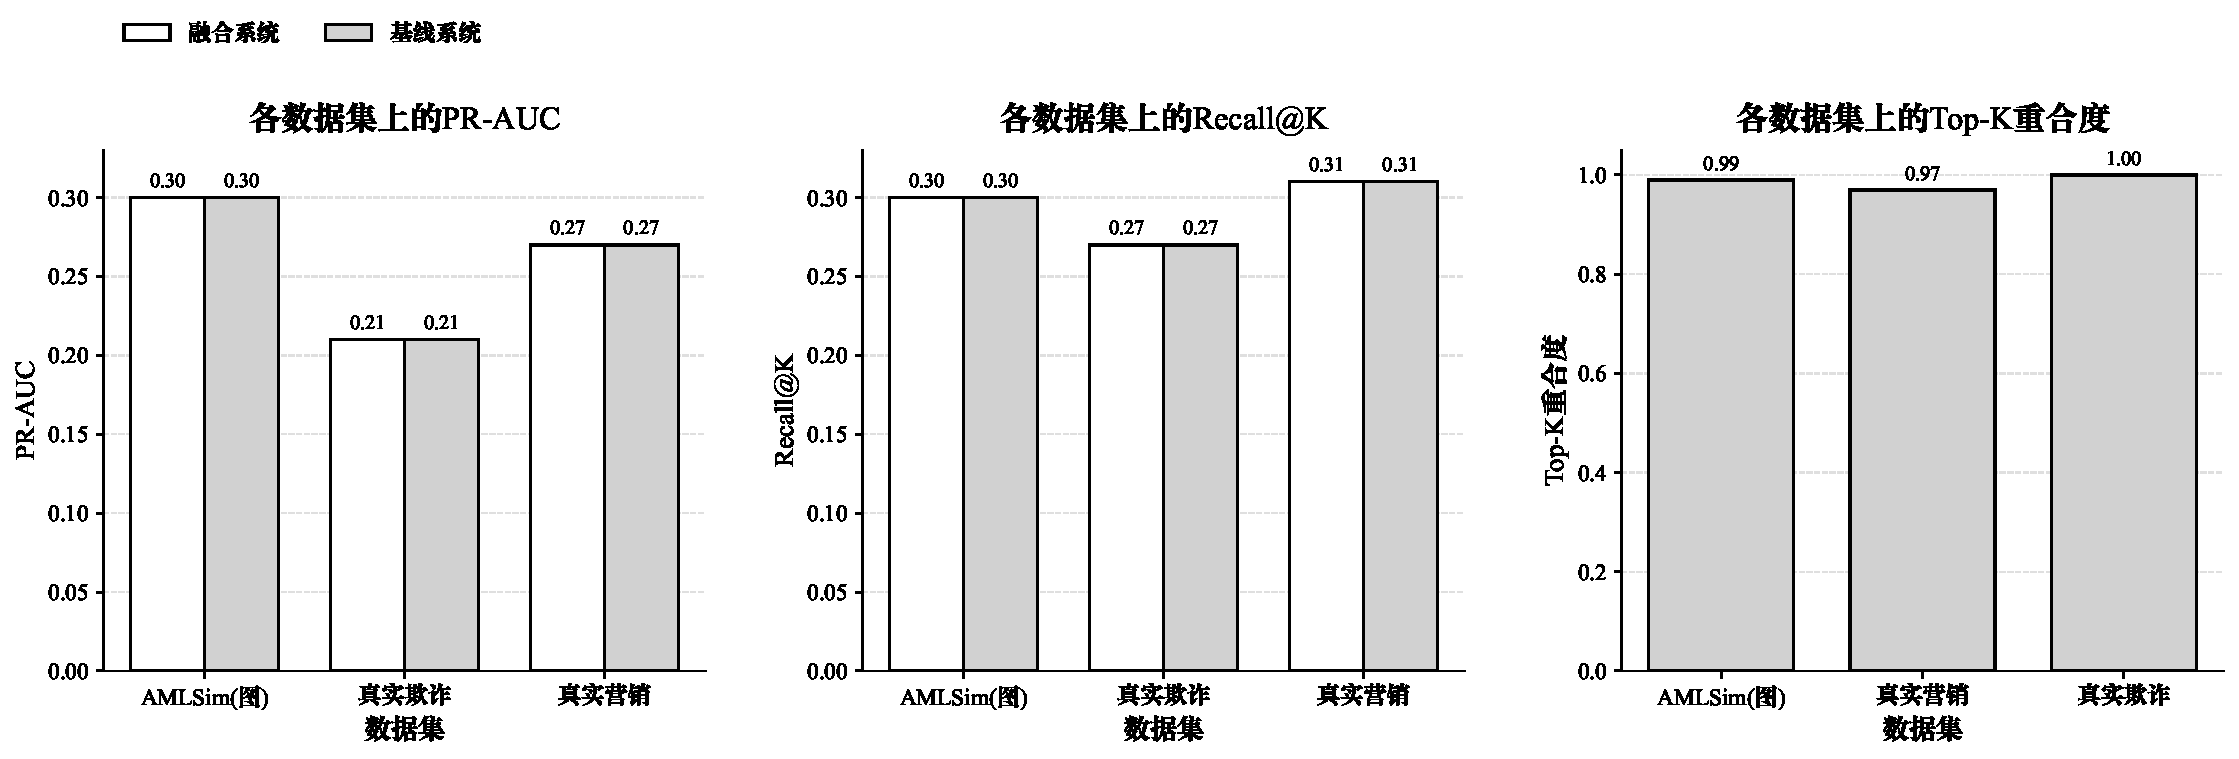
\includegraphics[width=\linewidth]{figures/fig3-6_initial_effectiveness_across_datasets.pdf}
  \caption{不同数据集上的候选召回---候选评分初步有效性验证结果（实验数据绘制）}
  \label{fig:prelim-effectiveness}
\end{figure}

\FloatBarrier

\section{本章小结}

本章围绕 FlashTOD 的功能结构，完成了任务建模、数据集选取、预处理与特征构造、异常评分模块设计、候选召回模块设计以及执行流程构建。通过对金融异常检测任务的统一抽象，本文将表格型金融数据与图金融数据共同映射为统一向量接口，并建立了``候选召回---异常评分''的两阶段处理框架。在实验准备上，本章进一步明确了全文统一的数据规模口径，使真实有效性验证、桥接实验、单卡性能分析和多 GPU 压力测试能够沿同一规模链路展开，从而为后续章节中的单卡优化和多 GPU 验证提供一致的数据基础。

本章解决了系统对象如何建立、模块接口如何对齐、基础实验如何起步的问题，但数据路径成本仍待处理。PyTOD 与 FlashANNS 已被放置在一条候选召回---异常评分执行链路中统一考察；当前链路主要满足功能可行和接口联通，尚未从系统层面压缩 CPU$\leftrightarrow$GPU 数据往返与阶段同步开销。因此，第四章将进一步进入单卡优化，重点讨论 GPU 主导执行链路、异步 I/O---计算流水线以及数据路径压缩问题。
